\chapter{Mise en œuvre et résultats} 

\lettrine{M}{aintenant} que le modèle est posé et que l'on sait quelles méthodes utiliser pour la calibration et le choix des solutions, on peut procéder.

La première étape à effectuer est l'analyse de sensibilité.
Il faut cependant au préalable définir les intervalles dans lesquels évoluent nos paramètres.
Si pour certains paramètres, les intervalles semblent naturels à choisir comme l'intervalle $[0; 1]$ pour les probabilités, le choix d'intervalles pour certains paramètres comme $\gamma$ s'avère plus hasardeux.
Procédons paramètre par paramètre.

En premier lieu, le paramètre $\gamma$ qui, rappelons-le, correspond au coefficient de proportionnalité sur les inflorescences vivantes qui permet de déterminer le nombre de femelles exogènes arrivant dans chaque sous-parcelle à chaque date.
Ce paramètre est propre à notre modèle, on ne peut donc pas trouver d'estimation dans la littérature.
On peut fixer la borne inférieure de l'intervalle à 0, en partant du principe qu'une cécidomyie préfère rester dans le verger duquel elle émerge plutôt que de migrer dans un autre verger.
On fixera la borne supérieure à 1. Cela signifie qu'il ne peut pas y avoir plus de femelles exogènes qui arrivent dans le verger que ce qu'il n'y a d'inflorescences.

Ensuite, par définition du paramètre $p_{\text{m}}$ (qui régule les échanges de femelles entre les trois sous-parcelles), on sait qu'il évolue dans l'intervalle $[0;1]$.
De la même manière, $\mu_{\text{ER}}$ et $\mu_{\text{EH}}$ désignent les probabilités de survie aux modalités de couverture du sol ER et EH.
Leurs intervalles seront donc aussi $[0;1]$.

Le paramètre $k$ relatif à la disponibilité en ressources gère le nombre d'attaques de cécidomyies que peut subir une attaque chaque jour.
Une inflorescence ne peut pas supporter trop d'attaques pour qu'elle ait une durée de vie qui ne soit pas extrêmement courte. On fixera le seuil supérieur à 2.
On sait aussi que quand l'inflorescence est jeune, elle particulièrement sensible aux attaques.
On fixera le seuil inférieur à 0.01.

Le \texttt{stock} d'individus en diapause sera fixé de manière assez large, dû à une absence d'estimation, entre 500 et 20000.

Enfin, le nombre d'œufs pondus qui survivent $E_0\mu_\ell$ est présent dans la littérature \citep{paul}.
Sa valeur est de 6, mais nous paraît peu fiable.
On le calibrera autour de cette valeur, entre 1 et 11.

Les intervalles étant définis, on peut maintenant faire l'analyse de sensibilité. Les résultats, pour un échantillon de taille $N = 50000$, sont visibles sur la figure~\ref{fig:sa}.

\begin{figure}
 \centering
 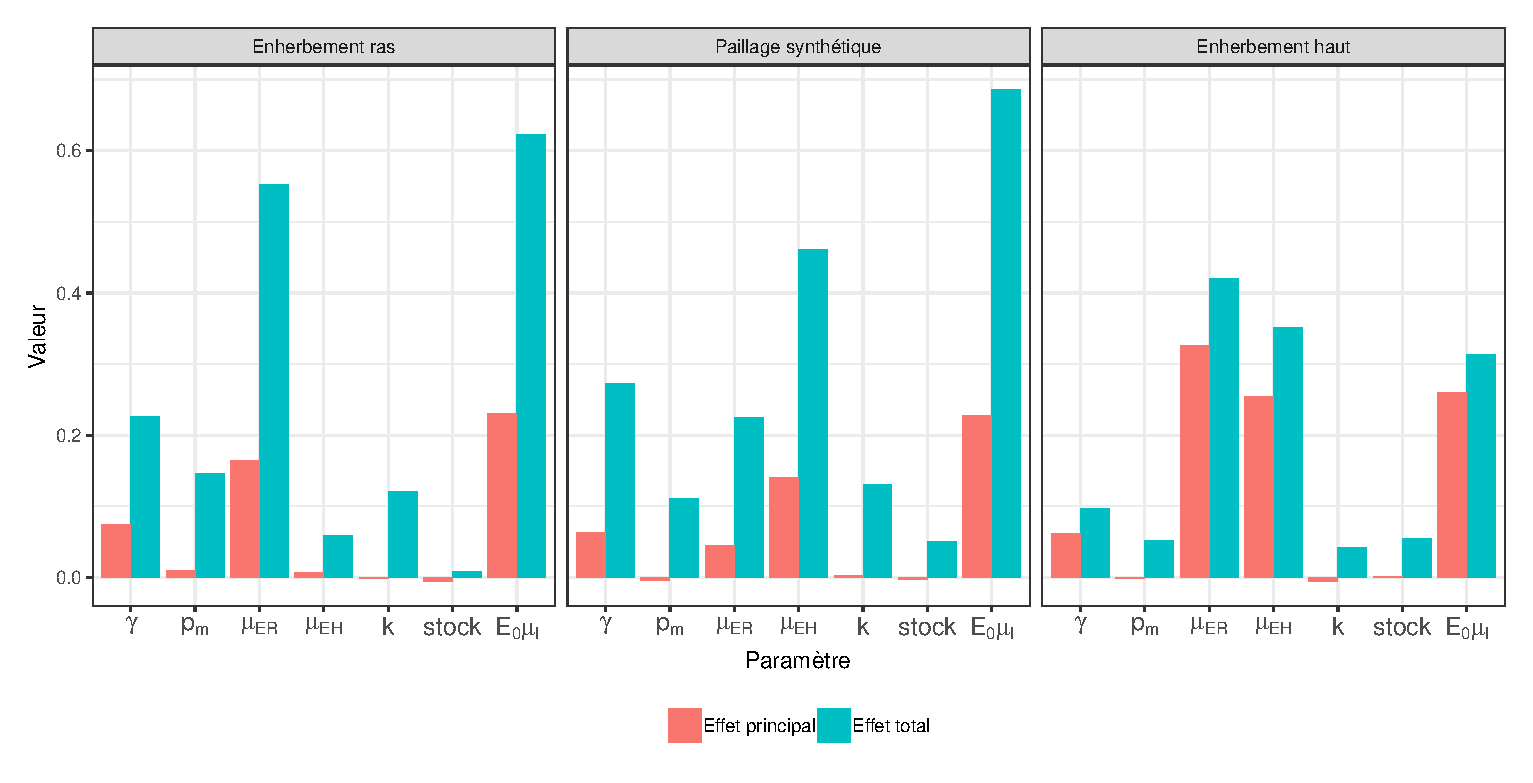
\epsfig{file = plots/sensitivity_analysis_A.eps, scale = 0.59}
 \caption{Analyse de sensitivité de notre modèle avec la méthode Sobol.}
 \label{fig:sa}
\end{figure}

On s'aperçoit que le paramètre apportant le plus de variance à la sortie de notre modèle (effet principal) est $E_0\mu_\ell$, et ce pour chacun des trois sous-parcelles.
Viennent ensuite les probabilités de survie à la modalité de couverture du sol.
Sans surprise, le paramètre $\mu_{\text{EH}}$ apporte beaucoup de variance à la sous-parcelle avec la modalité de couverture de sol correspondante.
De façon moins intuitive, ce paramètre apporte aussi beaucoup de variance à la sous-parcelle avec un enherbement haut.
Il y apporte même plus de variance que le paramètre $\mu_{\text{EH}}$, bien que ce dernier en apporte aussi une part importante.
Concernant la sous-parcelle avec un paillage synthétique, les probabilités de survie aux modalités de couverture du sol apporte aussi de la variance, avec un avantage pour $\mu_{\text{EH}}$.
À noter que le paramètre $\gamma$ n'est pas en reste non plus, induisant une part non-négligeable de variance sur chacune des trois-sous-parcelles.
Les paramètres $p_{\text{m}}, k$ et \texttt{stock} n'apportent en eux-mêmes que peu de variance.

On remarque également que les paramètres qui apportent le plus de variance sont aussi ceux dont les interactions induisent le plus de variance. (La variance apportée par les interactions d'un paramètre correspond à la différence entre l'effet total et l'effet principal).

Certains de ces résultats ne sont pas surprenants outre-mesure.
Il faut notamment se rappeler que le modèle est évalué sur l'estimation du nombre de larves, et que $E_0\mu_\ell$ intervient dans l'équation du modèle donnant le nombre de larves.
Ainsi, ce paramètre seul --- à valeur entre 1 et 11 --- peut facilement doubler le nombre de larves en fonction de sa valeur. Et induit donc naturellement une forte variance dans le modèle.
Et ce paramètre n'est interprétable que si l'on considère la valeur des autres paramètres.
Car un nombre élevé d'œufs pondus qui survivent peut être compensé par une faible probabilité de survie aux modalités de couverture de sol et une faible arrivée d'individus exogènes --- et vice-versa.
Ce qui peut expliquer ses fortes interactions.
Ce qu'il est bon de retenir de cette analyse de sensibilité concerne plutôt l'impact des probabilités de survie aux modalités de couverture du sol en fonction de chaque sous-parcelles, qui ne respecte pas ce que l'on pourrait s'imaginer \emph{a priori}.
Il est également bon de retenir que trois de paramètres ($p_{\text{m}}, k$ et \texttt{stock}) n'ont qu'un impact très limité --- comparativement aux autres --- sur la sortie du modèle.

Sachant cela, on peut utiliser NSGA-II pour obtenir un sous-ensemble du front de Pareto contenant des jeux de paramètres produisant des solutions non-dominées.
L'algorithme est cependant stochastique, il ne renvoie jamais exactement deux fois les mêmes résultats.
Pour pallier cet aspect, on exécute trente fois la fonction \texttt{nsga2} \citep{nsga} (avec une taille de population de 200, et 200 générations).
Cela nous donne ainsi 6000 solutions. Mais parmi ces 6000 solutions certaines sont peut-être dominées par d'autres solutions provenant d'une exécution de \texttt{nsga2} différente.
On ne récupère alors que les solutions non-dominées (et les jeux de paramètres correspondants) grâce à la fonction \texttt{is\textunderscore dominated} \citep{emoa}.
On obtient ainsi 842 jeux de paramètres produisant autant de solutions non-dominées.

On peut maintenant essayer de repérer différentes solutions--types reproduisant les quantités de larves observées.
On utilisera la fonction \texttt{hclust} \citep{R}.
Il faut dans un premier temps choisir un nombre de classes.
À cette fin, on regarde l'inertie intra-classes en fonction du nombre de classes (voir figure~\ref{fig:caha}).

\begin{figure}[ht]
 \centering
 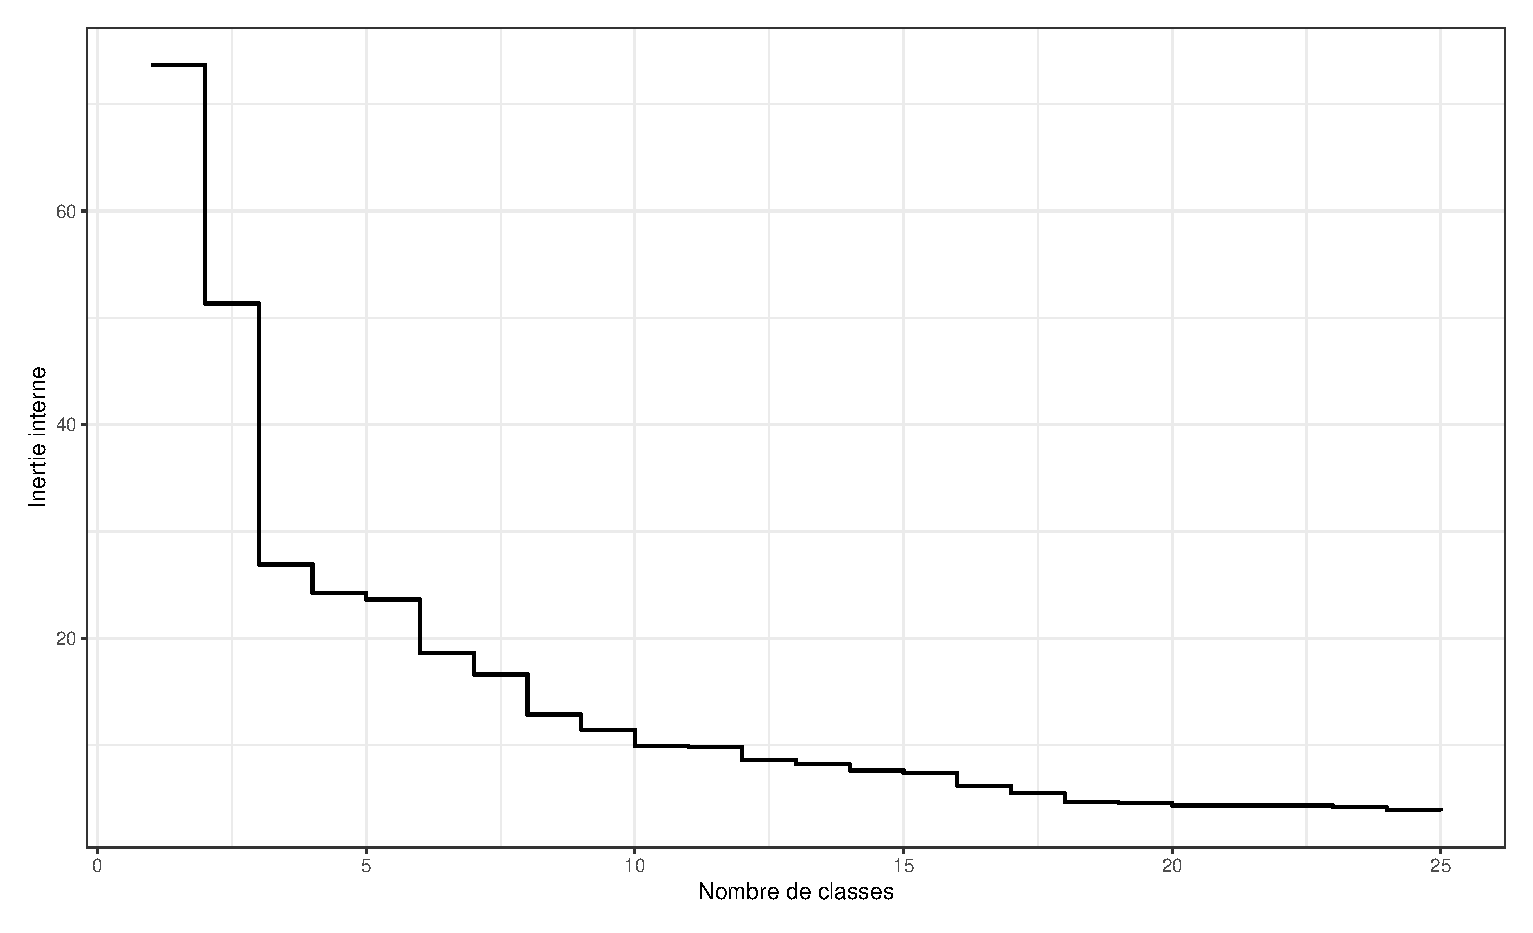
\epsfig{file = plots/cah_A.eps, scale = 0.55}
 \caption{Inertie intra-classes en fonction du nombres de classe obtenue par une CAH sur les jeux de paramètres renvoyés par NSGA-II.}
 \label{fig:caha}
\end{figure}

Dans une optique de classification «classique», choisir 2, 3, 6 ou 8 classes pourrait s'avérer pertinent.
(Ces nombres de classes produisant une minimisation relativement importante de l'inertie intra-classes.)
Nous préférons cependant ne pas risquer de passer à côté d'une catégorie de solution potentiellement intéressante.
Nous choisirons 16 classes.

Parmi les 16 classes, on distingue trois principales catégories de solutions.
Les voicis :
\begin{itemize}
 \item \textbf{Scénario 1 :} On observe des dynamiques (figure~\ref{fig:A1}) reproduisant grossièrement les dynamiques observées. 
 On observe une forte proportion de femelles exogènes, en particulier sur les sous-parcelles PS et EH, ce qui peut sembler invraisemblable.
 Les paramètres associées à ces trois dynamiques sont :
 \begin{center}
\begin{tabular}{lllllll}
$\gamma$ & $p_{\text{m}}$ & $\mu_{\text{ER}}$ & $\mu_{\text{EH}}$ & $k$ & \texttt{stock} & $E_0\mu_{\ell}$\\
0.08 & 0.494 & 0.976 & 0.046 & 1.928 & 5600 & 3.084
 \end{tabular}
 \end{center}
Les valeurs confirment le ressenti que l'on pouvait avoir. 
À savoir qu'il y a peu d'individus endogènes (les seuls présents sont issus de la sous-parcelle avec un enherbement ras).
\item \textbf{Scénario 2 :} C'est une solution sans femelles exogènes.
On remarque cependant que là encore, les individus endogènes ne proviennent que de la sous-parcelle ER.
Il en résulte que la simulation sur cette sous-parcelle est mauvaise. 
Il semble qu'elle ne sert uniquement de fournisseur de ravageurs aux deux autres parcelles, dont les dynamiques sont plus ou moins bien captées par le modèle.
Les paramètres sont :
 \begin{center}
\begin{tabular}{lllllll}
$\gamma$ & $p_{\text{m}}$ & $\mu_{\text{ER}}$ & $\mu_{\text{EH}}$ & $k$ & \texttt{stock} & $E_0\mu_{\ell}$\\
0 & 0.968 & 1 & 0.025 & 0.1 & 14483 & 6.26
 \end{tabular}
 \end{center}
Ce jeu de paramètres confirme la forte proportion d'individus exogènes dans la sous-parcelle ER avec une probabilité de de survie à ladite modalité égale à 1 et un gros stock d'individus en diapause.
Son rôle de fournisseur est confirmé avec un $p_{\text{m}}$ proche de 1.
Si l'absence totale d'individus exogènes est probablement erronée, ce qui reste le plus invraisemblable est cette absence d'individus qui émergent de la sous-parcelle avec un enherbement haut.
\item \textbf{Scénario 3 :} Il y a ici des individus exogènes dans la sous-parcelle EH.
Il faut cependant reconnaître que les dynamiques sont assez mal captées.
Les paramètres sont :
 \begin{center}
\begin{tabular}{lllllll}
$\gamma$ & $p_{\text{m}}$ & $\mu_{\text{ER}}$ & $\mu_{\text{EH}}$ & $k$ & \texttt{stock} & $E_0\mu_{\ell}$\\
0.026 & 0.93 & 0.565 & 0.647 & 0.174 & 13823 & 4.818
 \end{tabular}
 \end{center}
\end{itemize}

Ces trois scnénarios semblent tous montrer que le modèle tel qui est n'est pas suffisament complet pour capter le phénomène observé.
Il fait soit appel à trop d'exogènes, soit il n'y a aucun individus qui émergnent de la sous-parcelle EH, soit les deux.
Et lorsqu'il y a des indivdus qui émergent de la sous-parcelle EH, le modèle ne parvient pas à recréer les dynamiques observées.

Cela peut s'expliquer par l'incapacité pour le modèle d'arrêter la reproduction des femelles et donc de stopper la dynamique en fin de saison induisant la baisse du nombre de larves observé.


\begin{figure}
 \centering
 \textbf{Scénario 1}
 
 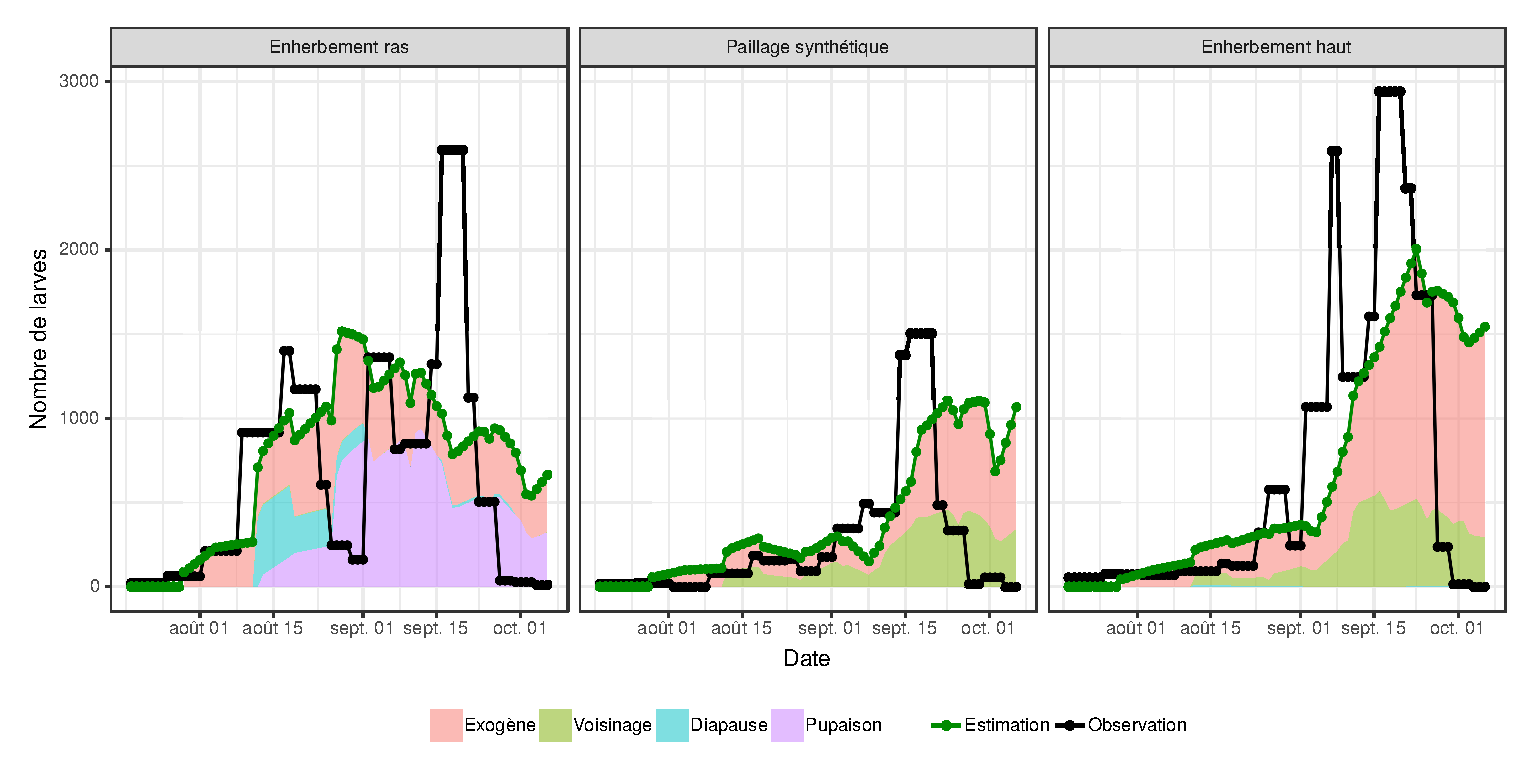
\epsfig{file = plots/A1.eps, scale = 0.55}
 
 \textbf{Scénario 2}
 
 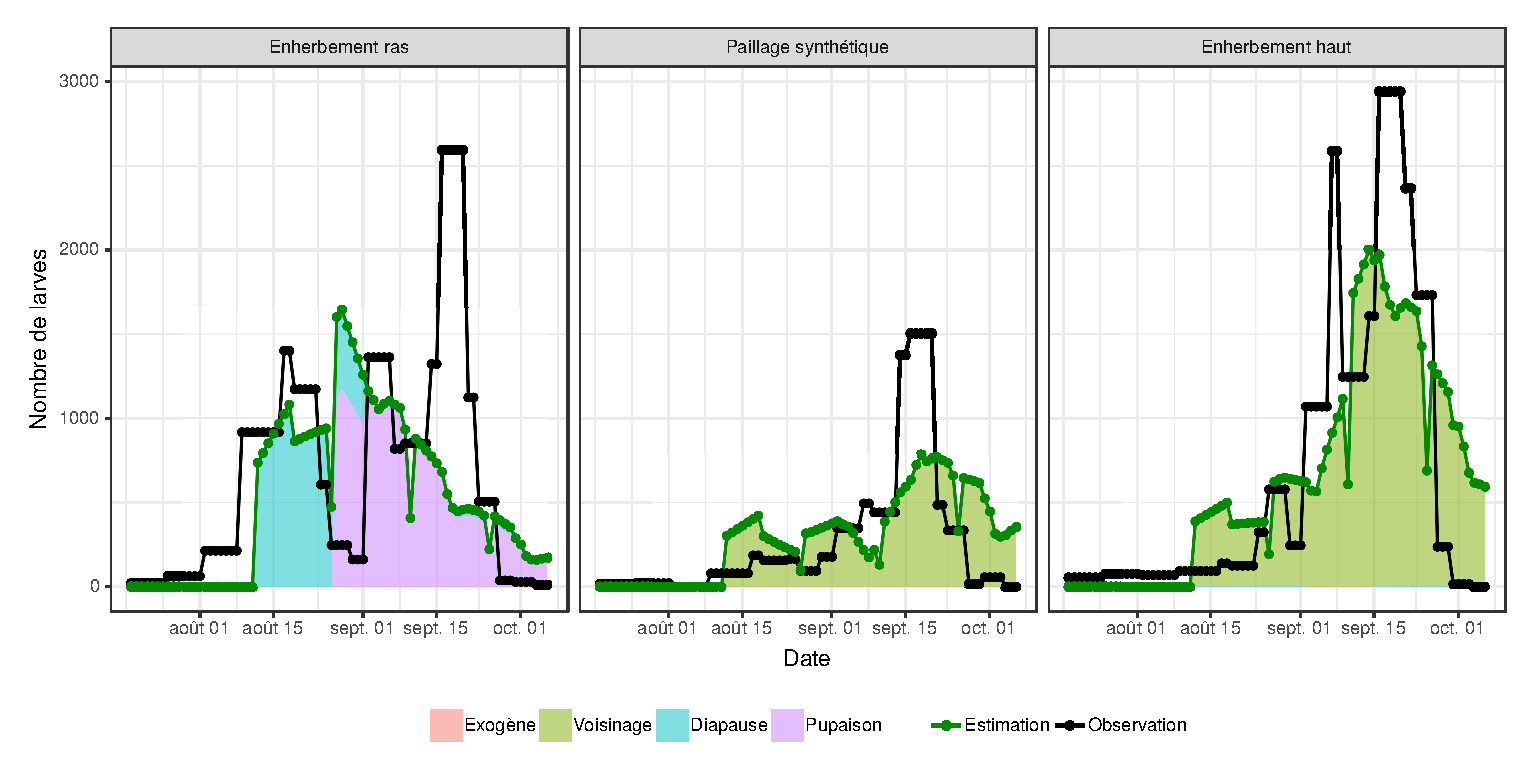
\epsfig{file = plots/A3.eps, scale = 0.55}
 
 \textbf{Scénario 3}
 
 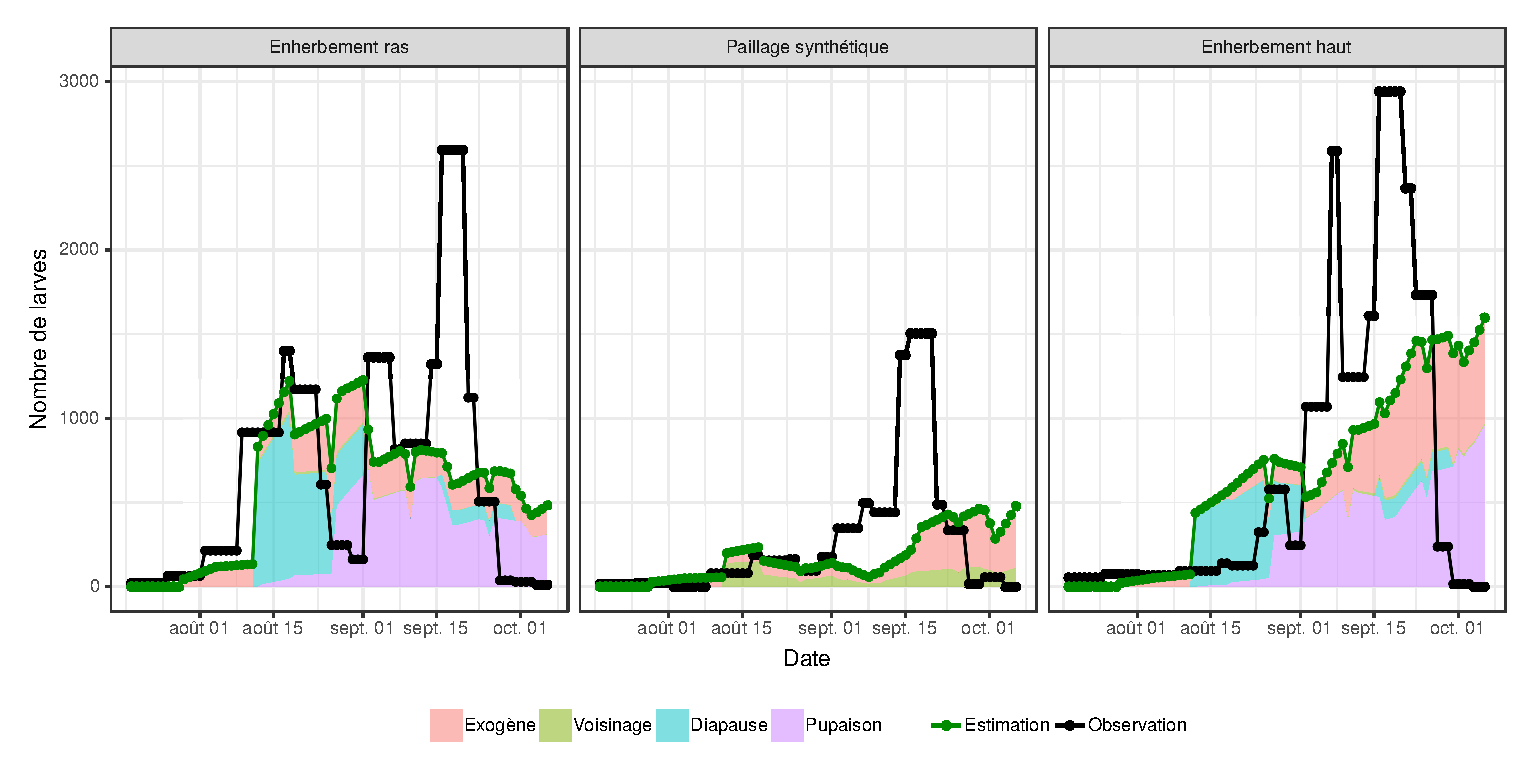
\epsfig{file = plots/A2.eps, scale = 0.55}
 \caption{Dynamiques observées et simulées pour chacun des trois scénarios. La décomposition indiquant la provenance des femelles qui ont pondus les œufs est disponible pour les dynamiques simulées.}
 \label{fig:A1}
\end{figure}










